\section{Experimental Evaluation}\label{sec:evaluation}

An Acting system, the Robustness Heuristics and the task preparations were implemented directly inside the system Fape \citep{bit-monnotFAPEConstraintbasedPlanner2020}.
The Statement around Fape supporting acting made in \cite{bit-monnotTemporalHierarchicalModels2016a} were not present in the current system as they have only been discussed theoretically or parts were deleted because of a domain-dependent implementation.
Due to technical difficulties, the planning of tasks by interleaving with already planned tasks and replanning could not be implemented in time.
Evaluation regarding these parts is done manually.

We consider four different variants of our domain definition:
\begin{itemize}
  \item Full Hier.: All action templates are task-dependent and the duration of the action template \verb|a_move| is fixed at 5.
  \item Full Hier. + Dur: All action templates are task-dependent and the duration of the action template \verb|a_move| is the shortest distance in the map calculated using the A* search algorithm. 
  \item Part. Hier.: The action template \verb|a_move| is not task-dependent, so agents can move freely in the domain if necessary and the duration of the action template \verb|a_move| is fixed at 5.
  \item Part. Hier. + Dur: The action template \verb|a_move| is not task-dependent, so agents can move freely in the domain if necessary and the duration of the action template \verb|a_move| is the shortest distance in the map calculated using the A* search algorithm. 
\end{itemize}

The evaluation was done in an LXC container with 12 Intel(R) Xeon(R) Gold 6334 CPU 3.60GHz Cores, 32 GB RAM.
Planning in FAPE is however a single-threaded process, so only one CPU Core can be used.

% Quantitative Metrics:
% Plan time
% Search Nodes
% Average Branching Factor

% Makespan/Duration

% Qualitative Metrics:
% Success

% Possible Comparisons:
% HTN PO vs HTN TO vs Classical \citep{yuxinliuPlanningOvercookedGame2020}
% HTN vs HTN + Robustness
% HTN Oracle vs HTN Acting vs HTN Acting + Robustness vs HTN + Preparations

\subsection{Environments}

We consider two environments in this evaluation.


\bild{fig:eval-overcooked}{overcooked2_tutorial}{Overcooked!2 Tutorial level}{10}

First, we consider the ``tutorial level'' of the ``Overcooked!2'' game shown in Figure \ref{fig:eval-overcooked}.
Version 2 of ``Overcooked'' adds only the functionality to toss items, more levels and more recipes.
Since tossing items is not considered here, it makes no difference which version of the game is used.
The environment provides the three ingredients lettuce, tomato and cucumber, the tableware plate and the tool knife.
The orders that may be received are a simple salad, consisting of only lettuce, a lettuce tomato salad and lastly a salad with lettuce tomato and cucumber.
All of the ingredients have to be chopped using a knife before they are assembled on a plate.
Each ingredient and tableware is present five times, there are four knives and two cooks available.
The map has a narrow path to get to the locations of the knives.
We define four possible arrange areas, two in the middle on each side and two on the bottom on each side.

\bild{fig:eval-mapB}{pddl_mapB}{Map}{10}

Second, we consider the ``complex map'' shown in Figure \ref{fig:eval-mapB} from \cite{yuxinliuPlanningOvercookedGame2020}.
This environment is not from the official game.
It provides the ingredients beef, lettuce, tomato and burger bun, the tableware plate and the tools knife and pan.
The orders received here are burgers with a burger bun, a steak, lettuce and tomato.
The lettuce and tomato have to be chopped and the steak fried in the pan before they are assembled on a plate.
Each ingredient and tableware is again present five times, there are two knives, two pans and two cooks available.
The map has a long counter and cooks must walk around it to move between the ingredient locations and the tools, so the cooks are encouraged to pass ingredients over the counter.
There are two arrange areas at the same place as seen in Figure \ref{fig:eval-mapB}. 

\subsection{HTN vs Classical Planning in Overcooked}


In this section, we compare our HTN domain definition for ``Overcooked'' with the PDDL domain definition by \cite{yuxinliuPlanningOvercookedGame2020}.
It is not possible to directly compare the makespan between the domains, as not all of the action durations were provided.
To plan using the HTN domain definition, we use FAPE \citep{bit-monnotTemporalHierarchicalModels2016a} and they use the Temporal Fast Downward planner \citep{eyerichUsingContextenhancedAdditive2009}.
The environment is the ``complex map'' shown in figure \ref{fig:eval-mapB}.
The goal of this problem is to prepare either one or two burgers.


It is important to note that FAPE uses different heuristics by default during planning compared to TFD.
FAPE uses the heuristic minimal spanning tree for partially hierarchical domains and depth-first search in fully hierarchical domains.
While the selection of different heuristics is possible in FAPE, it is not considered in this comparison.
\cite{yuxinliuPlanningOvercookedGame2020} uses the shortest makespan heuristic.
As such, FAPE only does satisficing while TFD tries to find the optimal plan.

Additionally, TFD uses State-Space search while FAPE uses Plan-Space search.
This makes the generated nodes not directly comparable.

The results of planning the delivery of one burger are shown in Table \ref{tab:eval-burger}.
TFD is faster in the generation of the plan and visits significantly more nodes than FAPE.
The search time for the partial hierarchy is also slower than the fully hierarchal version.
The inclusion of the representative movement durations also increases the search time for both variants.
The makespan is however shorter for the partial hierarchy compared to the full hierarchy, especially when using the representative movement durations.


\begin{table}
  \centering
  \begin{tabular}{lcllll}
                   & Success & search time  & generated nodes & makespan         \\
    \hline
    TFD             & yes & $20s$            &  10546          &  125.1       \\
    Full Hier.            & yes & $31.0s\pm 0.9$   & $125\pm 0.0$    &  $232\pm 0.0$            \\
    Full Hier. + Dur      & yes & $37.9s\pm 1.6$   & $125\pm 0.0$    &  $368\pm 0.0$      \\
    Part. Hier.      & yes & $563.0s\pm 45.1$ & $3754\pm 0.0$   &  $227\pm 0.0$   \\
    Part. Hier. + Dur & yes & $628.0s\pm 16.9$ & $3744\pm 0.5$   &  $318\pm 0.0$            \\
  \end{tabular}
  \caption{Produce one burger}
  \label{tab:eval-burger}
\end{table}

The results for planning the delivery of two burgers are shown in Table \ref{tab:eval-burgers}.
Both planners are unable to find a solution in this case.
TFD does consider more search nodes than FAPE, as in the previous comparison.

\begin{table}
  \centering
  \begin{tabular}{lcllll}
    & Success & search time  & generated nodes & makespan         \\
  \hline
  TFD             & no & $1000s+$ & 1000000+ &  -       \\
  FAPE            & no & $1000s+$ & 5360+    &  -          \\
  FAPE + Dur      & no & $1000s+$ & 7430+    &  -    \\
  FAPE + TI       & no & $1000s+$ & 3800+    &  - \\
  FAPE + Dur + TI & no & $1000s+$ & 3071+    &  -          \\
  \end{tabular}
  \caption{Produce two burgers}
  \label{tab:eval-burgers}
\end{table}

\subsection{Robustness Heuristic}

In this section, we evaluate the Robustness Heuristic introduced in Section \ref{sec:approach-robustness}.
Heuristics can be provided as a list in FAPE, to assign a priority.
The additional heuristics are used to break ties between previous heuristics.

The default heuristics used are depth-first search (``dfs''), ordered decomposition (``ord-dec'') and ``soca'' which is a simple comparison between the number of flaws and actions.
We compare this default heuristic with four different combinations of adding either the shortest makespan or the robustness heuristic at index 2 or 3.
The depth-first search should always be at the first index for fully hierarchical problems, as the search would otherwise not resolve tasks first.


We compare the heuristic combinations in the following four different simple problems using the ``Full Hier. + Dur'' domain.
The environment for the salads is the ``tutorial level'' (see Figure \ref{fig:eval-overcooked}).
For the burger it is the ``complex map'' (see Figure \ref{fig:eval-mapB}).
\begin{enumerate}
  \item a lettuce salad, with a deadline of 150:\\ 
    \verb|[start, start+150] contains order_po_lettuce_salad(client1);|
  \item two lettuce salads, with a deadline of 300 each:\\
    \verb|[start, start+300] contains order_po_lettuce_salad(client1);|\\
    \verb|[start, start+300] contains order_po_lettuce_salad(client2);|\\
  \item a tomato salad with a deadline of 200:\\
    \verb|[start, start+200] contains order_po_lettuce_tomato_salad(client1);|
  \item a burger with a deadline of 200:\\
    \verb|[start, start+400] contains order_po_lettuce_tomato_burger(client1);|
\end{enumerate}

\begin{table}[]
  \centering
  \begin{tabular}{p{1.5cm}rrrrr}
  \multicolumn{1}{l}{}         & \multicolumn{1}{l}{heuristic} & success & \multicolumn{1}{l}{plantime} & \multicolumn{1}{l}{generated states} & \multicolumn{1}{l}{makespan} \\ \hline \hline
  \multirow{5}{*}{salad}        & default                       & yes     & $11.8s\pm1.5 $              & $46.0\pm0.0$                         & $115.0 \pm0.0$               \\ 
                                & makespan@2                    & yes     & $11.4s\pm1.5 $              & $53.0\pm0.0$                         & $79.0  \pm0.0$               \\ 
                                & makespan@3                    & yes     & $11.1s\pm1.7 $              & $53.0\pm0.0$                         & $79.0  \pm0.0$               \\
                                & robustness@2                  & yes     & $11.6s\pm1.3 $              & $48.6\pm5.3$                         & $110.6 \pm25.5$               \\ 
                                & robustness@3                  & yes     & $11.7s\pm1.3 $              & $45.8\pm2.5$                         & $115 \pm21.2$               \\\hline
  \multirow{5}{*}{\parbox{1.2cm}{two salads}}   
                                & default                       & no      & $1000.0s+$                  & $39641.0\pm?$                        & $-     $                     \\
                                & makespan@2                    & no      & $1000.0s+$                  & $38906.2\pm1541.4$                   & $-     $                     \\
                                & makespan@3                    & no      & $1000.0s+$                  & $36023.0\pm554.3$                    & $-     $                     \\
                                & robustness@2                  & no      & $1000.0s+$                  & $16584.0\pm?$                        & $-     $                     \\ 
                                & robustness@3                  & no      & $1000.0s+$                  & $21336.0\pm?$                        & $-     $                     \\\hline
  \multirow{5}{*}{\parbox{1.5cm}{tomato salad}} 
                                & default                       & yes     & $10.8s\pm1.5 $              & $75.0\pm0.0$                         & $180.0 \pm0.0$               \\
                                & makespan@2                    & yes     & $12.0s\pm0.3 $              & $119.0\pm0.0$                        & $118.0 \pm0.0$               \\
                                & makespan@3                    & yes     & $12.0s\pm0.2 $              & $115.0\pm0.0$                        & $121.0 \pm0.0$               \\
                                & robustness@2                  & yes     & $15.0s\pm2.7 $              & $171.4\pm39.4$                           & $175.4 \pm2.2$               \\
                                & robustness@3                  & yes     & $12.1s\pm1.8 $              & $79.2\pm4.3$                            & $190.2 \pm3.9$               \\\hline
  \multirow{5}{*}{burger}       & default                       & yes     & $38.1s\pm 3.1$              & $125.0\pm0.0$                        & $368.0\pm0.0$                \\
                                & makespan@2                    & no      & $1000.0s+$                  & $5389.2\pm448.1$                     & $-     $                     \\
                                & makespan@3                    & no      & $1000.0s+ $                 & $5323.6\pm234.7$                     & $-     $                     \\
                                & robustness@2                  & yes     & $342.1s\pm365.2 $           & $2108.8\pm2462.0$                    & $329.4 \pm21.29$             \\ 
                                & robustness@3                  & 50\%    & $522.5s\pm675.4 $           & $1918.5\pm2535.0$                    & $358.0 \pm?$                                      
  \end{tabular}
  \caption[Performance results for different heuristic combinations]{Performance results for different heuristic combinations on different problems. The default heuristic is a priority combination with depth-first search (``dfs''), ordered decomposition (``ord-dec'') and ``soca'' which is a simple comparison between the number of flaws and actions. The other heuristic combinations in the table are created by inserting them at the respective index (starting at 1) in the priority combination, e.g. makespan@2 would result in the list (dfs,makespan,ord-dec,soca).}
  \label{tab:eval-heuristics}
\end{table}

The results are shown in table \ref{tab:eval-heuristics}.
Each heuristic variant was evaluated 5 times on each problem.
The arithmetic mean value is shown first and the standard deviation second.
When the standard deviation is $?$, the calculation of the standard deviation returned nan.

Producing a single salad takes only around 10 seconds for all of the heuristics.
The makespan heuristic combinations achieve a significant decrease in the makespan of the plan.
The makespan of the robustness heuristics is not better than the default and has a high standard deviation.

None of the heuristics can provide a plan for two salads at the same time in under 1000 seconds.
The default and makespan heuristics do however generate more states than the robustness heuristics.

All heuristics succeed with the tomato salad, the planning times are between 10 and 15 seconds, with the robustness@2 having the longest mean planning time at 15 seconds.
The highest number of generated states has the robustness@2 heuristic, while robustness@3 and the default heuristic generate a similar number of states.
The makespan values show a similar picture as with the simple salad.
The makespan heuristics have the shortest one, and the robustness heuristic ones are only not much different than the default one.

The burger is only planned successfully by the default heuristic and the robustness@2 heuristic.
The robustness@3 heuristic succeeds only partially \todo{how often?} in the 1000 seconds and the makespan heuristics do not finish.
The robustness@2 heuristic has however a very high standard deviation.
The default heuristic generates the lowest number of states, while the mean for the robustness@2 heuristic is much higher, but also with a very high standard deviation.
The highest number of states are generated by the makespan heuristics, but around 7 times fewer states than in the two salads problem in the same time frame.
The lowest makespan here is by the robustness@2 heuristic, but again with a high variance.

\todo[inline]{go in depth on an example for robustness}

\subsection{Acting}

In this section, we evaluate the impact of the robustness heuristic and the task preparations on acting.
We use the environment ``tutorial level'' in the ``Full Hier. + Dur'' domain with the following tasks:
\begin{itemize}
  \item \verb|[0,200] contains order_po_lettuce_tomato_salad(client1);|
  \item \verb|[100,300] contains order_po_lettuce_tomato_salad(client2);|
  \item \verb|[150,350] contains order_po_lettuce_tomato_salad(client3);|
\end{itemize}

Each task is received by the Activity Manager at the start of the temporal interval it is contained in.

We consider four different configurations:
\begin{itemize}
  \item default: no additional changes to FAPE
  \item makespan: the makespan@2 heuristic is used to get the shortest plan for each received task.
  \item preparations: the optimal preparations are inserted into the default plan.
  \item robustness: the robustness heuristic is used for generating a plan for each task
\end{itemize}

Acting is simulated by hand, by adding the optimal plans for the second and third tasks consecutively without replanning or repair.
This measures the ability of the configurations to find a plan without replanning or repair.
Since representative action durations are used, the durations for each action may be different.
We therefore use the optimal durations that are calculated with the makespan@2 heuristic for the first task.
These durations are: 
\begin{itemize}
  \item $dur(prep)=20$
  \item $dur(transport)=37$
  \item $dur(chop)=11$
  \item $dur(arrange)=18$
  \item $dur(deliver)=27$
\end{itemize}

The results are shown in Table \ref{tab:eval-acting} and a visual representation is shown in Figure \ref{fig:eval-acting}.
The task \verb|m_chop| was split into the two subtasks \verb|transport| and \verb|a_chop|, as they can be handled by different cooks. 

All of the configurations succeed in this manual evaluation with optimal task addition.
The makespan configuration represents the optimal configuration when not allowing preparations.
It has the highest margin for each task and the highest average margin.
It also has the shortest overall makespan.
The second best configuration is using the preparations with a lower margin for each task but a high margin for the second task.
The total makespan is also longer.
The robustness configuration has a higher margin than the preparations for the first task, but is lower for all others.
The total makespan is also only 3 time points lower than failure.
The default configuration has the lowest margins and reaches the deadline for task 3 just on time.

\begin{table}
  \centering
  \begin{tabular}{lrrrrrr}
                & success & \multicolumn{3}{c}{margin}  & avg margin     & total makespan  \\
                &         &  task 1 & task 2  & task 3  &                &  \\ \hline
  default       & yes     & $25$    & $32$    &  $0$    & $19$           & $350$     \\
  makespan      & yes     & $87$    & $87$    &  $58$   & $77.3$         & $292$       \\
  preparations  & yes     & $25$    & $62$    &  $19$   & $35.3$         & $331$    \\
  robustness    & yes     & $39$    & $46$    &  $3$    & $29.3$         & $347$ \\
  \end{tabular}
  \caption{Produce two burgers}
  \label{tab:eval-acting}
\end{table}



\begin{sidewaysfigure}
  \centering
  \subfloat[Default FAPE]{\label{fig:eval-acting-default}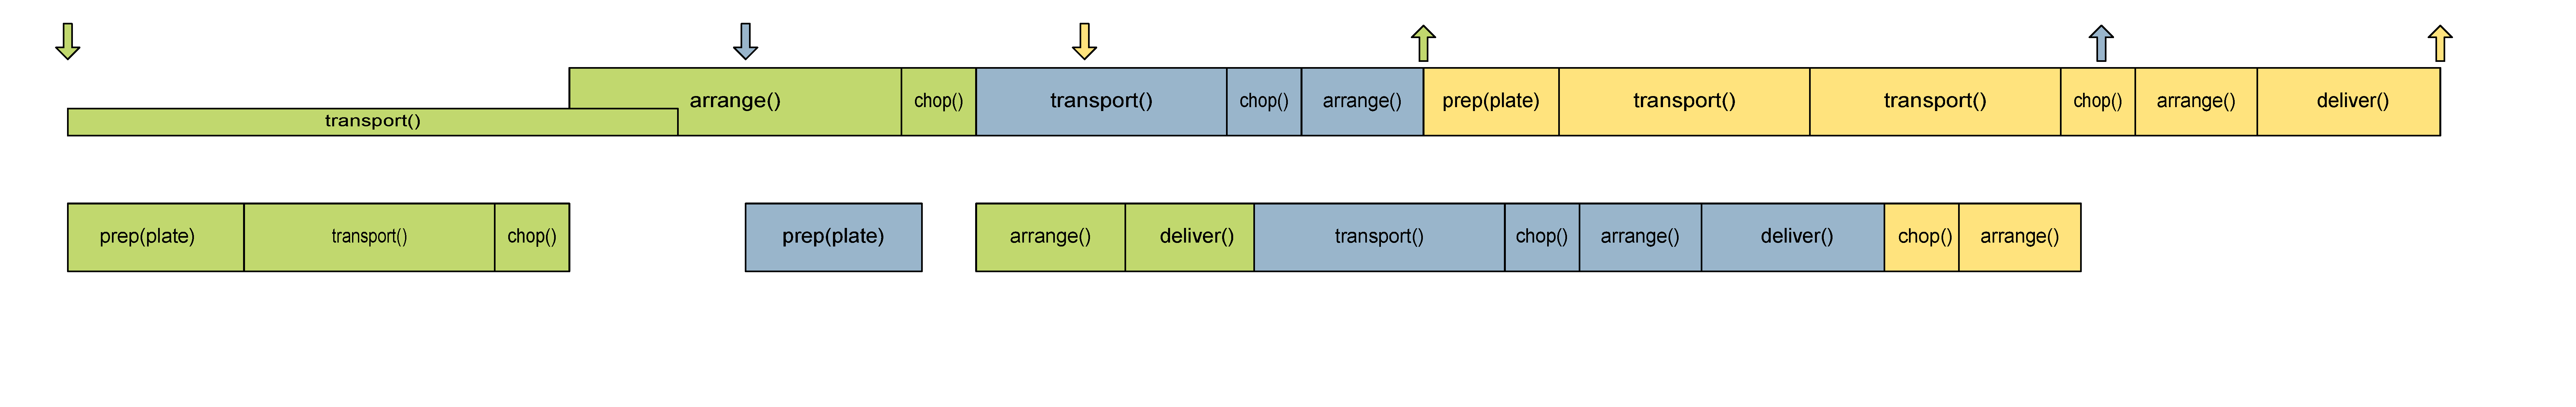
\includegraphics[width=\linewidth]{images/Scenario3 tomato - default.pdf}} \\\medskip
  \subfloat[Makespan Heuristic]{\label{fig:eval-acting-makespan}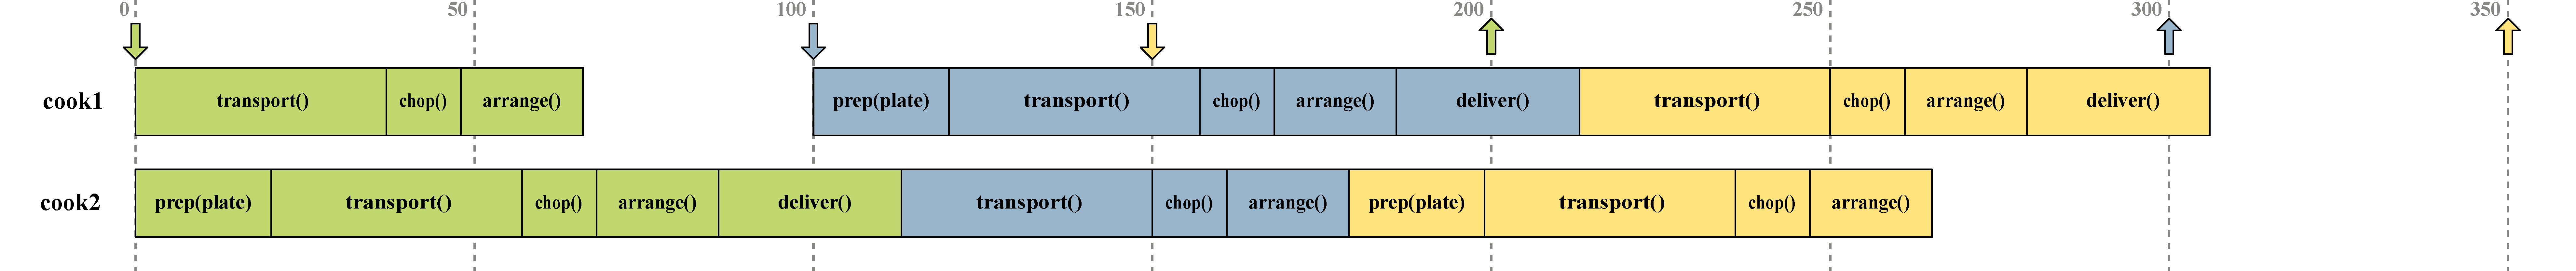
\includegraphics[width=\linewidth]{images/Scenario3 tomato - oracle_makespan.pdf}} \\\medskip
  \subfloat[Preparations, grey boxes represent inserted preparations]{\label{fig:eval-acting-preparations}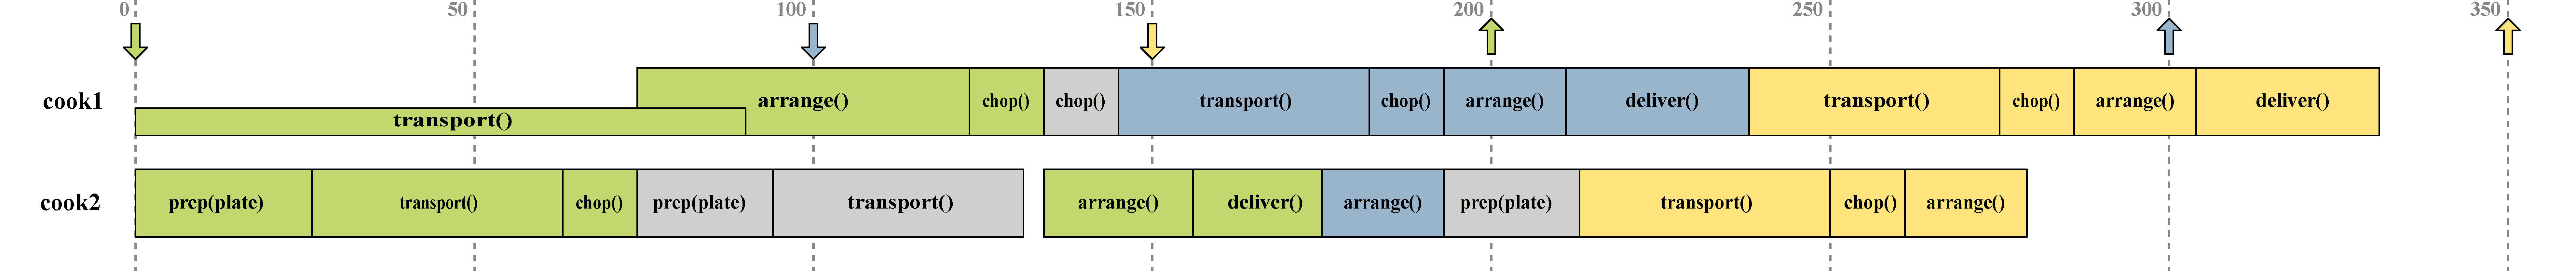
\includegraphics[width=\linewidth]{images/Scenario3 tomato - preparations.pdf}} \\\medskip
  \subfloat[Robustness Heuristic]{\label{fig:eval-acting-robustness}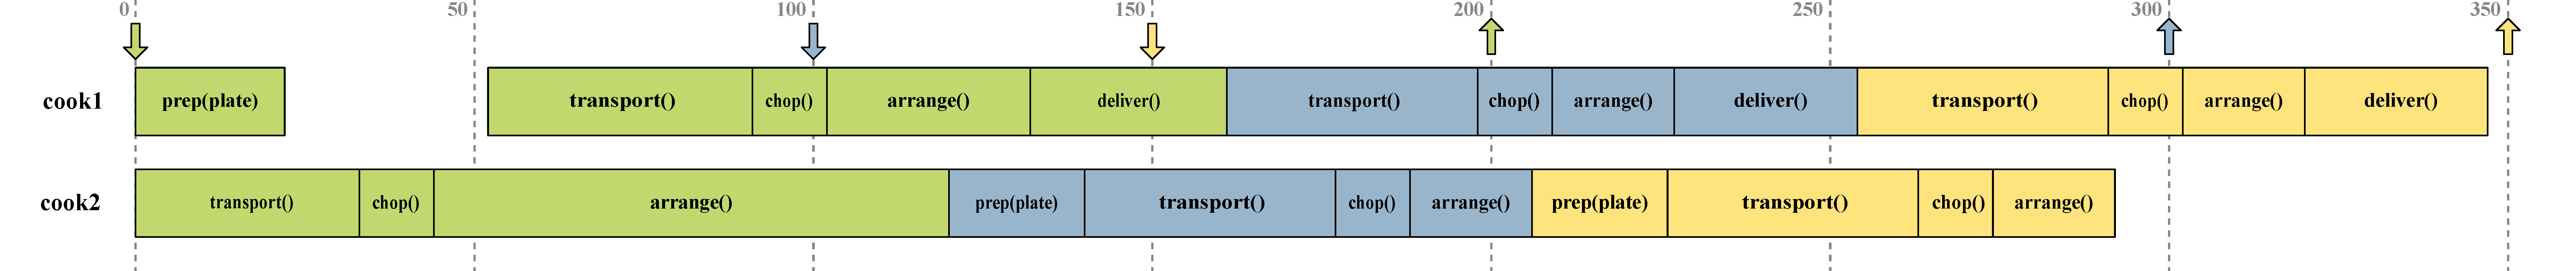
\includegraphics[width=\linewidth]{images/Scenario3 tomato - robustness.pdf}} \\\medskip
  \caption[]{Timeline-like representations of the plan executed by acting. Each row shows the actions performed by one of the cooks. Each color represents a task, the downpointing arrows represent the start time of a task and the uppointing arrows the deadline.}
  \label{fig:eval-acting}
\end{sidewaysfigure}
